\documentclass[11pt]{article}
\usepackage[margin=1.1in]{geometry}
\usepackage{amsmath,amssymb}
\usepackage{booktabs}
\usepackage{graphicx}
\usepackage[hidelinks]{hyperref}
\usepackage{xcolor}
\usepackage{pgfplots}
\pgfplotsset{compat=1.17}
\usetikzlibrary{arrows.meta,positioning}
\definecolor{accent}{RGB}{42,101,175}
\definecolor{corrupt}{RGB}{201,109,44}
\definecolor{inkmut}{RGB}{110,118,126}

\title{Design by Falsification:\\
an Evidence-Bound Multi-Agent Harness Distilled from a\\
Council of Experts That Mostly Did Not Work}
\author{Sam Bobo\\ \small with analysis assistance from Claude (Anthropic)}
\date{Draft v0.1 --- August 2026}

\newcommand{\ci}[2]{\ensuremath{[#1,\,#2]}}

\begin{document}
\maketitle

\begin{abstract}
We set out to build a council of experts: domain-specialist language
models feeding a lead writer, on the premise that specialists know
things generalists do not, that instructions can make the lead careful,
and that models can tell you when they are out of their depth. Across
more than fifty pre-registered experiment cells on auditable local
hardware (7--20B models), nearly every premise was falsified ---
specialist fine-tunes carry per-model, not per-domain, signatures; an
epistemic instruction installs only its named phrase; preference judges
then penalize that phrase; models' stable self-reports (confidence,
priors, ownership) do not predict their behavior; and prose transports
only $0.11$--$0.33$ of the epistemic qualification it is given. This
paper reports what happened next. The falsifications were themselves
findings, and they compose into an architecture: an orchestration
harness in which redundancy is engineered rather than hoped for,
epistemic freight travels outside the writer's prose, re-consultation
is triggered by mandated artifacts rather than self-assessment, and no
component survives on rationale alone. Every load-bearing design rule
was then re-tested prospectively as its own registered cell. Assigning
a contested quantity to a second specialist halves corrupted-value
adoption ($0.900\to0.450$); an appendix assembled outside the writer
carries $100\%$ of specialist caveats against the $17\%$ that survives
prose, flips downstream decisions ($+0.691$ over a matched irrelevant
control) at parity with in-prose placement, and shows no detected
preference cost; and the full re-consultation loop closes with a live
specialist ($0.905$ adoption vs.\ $0.333$ control, within noise of a
scripted ceiling). Two registered tests went \emph{against} our design
rationales --- sibling isolation lost its contamination warrant to an
informative null, and an elicited ownership law died in its
confirmation cell at exactly chance --- and the harness records both
demotions in place. We argue this is the correct acquisition path for
multi-agent architecture: not accumulating plausible components, but
keeping only what survives registered attempts to kill it.
\end{abstract}

\section{Introduction: the council that was supposed to work}
\label{sec:intro}

The plan was conventional wisdom circa 2024--2025. Take three
domain-specialist models --- healthcare, legal, finance --- have each
analyze a decision problem from its own expertise, and let a lead
writer synthesize their contributions. Aggregation pipelines of this
shape report state-of-the-art preference results
\cite{wang2024moa}; specialist fine-tunes are abundant; and the
architecture's premises feel almost too obvious to test: specialists
contribute what generalists cannot; instructing the lead to preserve
uncertainty makes it careful; a model that is out of its depth can say
so; corroboration among specialists strengthens claims.

We tested them. The program ran as a falsification-first ledger: every
cell pre-registered with predictions, falsification conditions, and
attainability computed from the archive before any run; every
deviation and verdict recorded; instruments themselves audited
(fourteen recorded instrument-validity findings). A companion paper
\cite{bobo2026audit} reports the audit findings in full. This paper
tells the systems story: \textbf{what it looks like to lose most of
your architecture's premises in public, and what you can build from
the parts that survive}.

The arc, compressed:

\begin{enumerate}
\item \textbf{The premises died} (\S\ref{sec:premises}). Not to opinion
--- to registered cells with pre-stated kill conditions, most of which
fired.
\item \textbf{The corpses were load-bearing} (\S\ref{sec:survivors}).
Each falsification localized a real mechanism: the lead is a source
selector, not a verifier; compliance is not behavior; the scarce
resource in consultation is the trigger, never the capability.
\item \textbf{The mechanisms compose into a harness}
(\S\ref{sec:harness}). If protection is coverage, engineer coverage. If
prose loses freight, do not ship freight in prose. If self-assessment
is empty, trigger from mandated artifacts instead.
\item \textbf{The harness was then attacked, component by component}
(\S\ref{sec:retests}). Six registered verdicts: four components
survived with causal or predictive effect sizes, one design rationale
was demoted by an informative null, and one candidate law was killed by
its own confirmation cell. The architecture that remains is smaller
than what we designed and better than what we assumed.
\end{enumerate}

\paragraph{Why this is a systems contribution.} Multi-agent frameworks
ship components on rationale: a verification stage because verification
sounds prudent, a confidence threshold because calibration sounds
measurable, a debate round because deliberation sounds epistemic. Our
central claim is methodological: \textbf{every component of a
multi-agent system is an empirical claim about model behavior, and most
such claims are false at the scale where practitioners actually deploy
them.} The harness presented here is not offered as the best possible
architecture. It is offered as the subset of one architecture that
survived fifty-plus registered attempts at its premises, with the
verdicts --- including the demotions --- attached to the components
they license.

\section{How the premises died}
\label{sec:premises}

Table~\ref{tab:premises} is the program's obituary column. Each row is
a premise the council needed, the registered cell that tested it, and
what happened. Effect sizes and protocols are in the companion paper;
here we give each one sentence of mechanism.

\begin{table}[t]
\centering\small
\begin{tabular}{p{0.34\textwidth}p{0.24\textwidth}p{0.32\textwidth}}
\toprule
premise the council needed & test & verdict \\
\midrule
Specialist fine-tunes share a domain signature & two medical tunes of
one base vs.\ their base & \textbf{falsified} --- signatures are
per-model; the tunes disagree with each other \\
An epistemic instruction changes the lead's behavior & counterbalanced
phrase-swap; synonym forms & \textbf{falsified} --- the named phrase
appears ($0.67$--$0.70$); the construct beyond it is unchanged
(CIs \ci{-0.079}{+0.111}, \ci{-0.103}{+0.087}) \\
Careful marking is at worst neutral under evaluation & order-debiased
preference, phrase arms vs.\ own control & \textbf{reversed} --- the
phrase \emph{loses} preference ($0.261$, $0.317$; replicated
cross-family) \\
A specialist can flag its own limits & roster + deferral token;
in- vs.\ out-of-domain & \textbf{falsified} --- routing is accurate
when fired ($0.909$) but discrimination spans zero ($0.306$ vs.\
$0.083$) \\
Corroboration among specialists strengthens transport & planted
agreement across contributions & \textbf{null} --- $0.487$ vs.\
$0.524$, CI spans zero \\
The lead verifies or recomputes & corrupted-source injection &
\textbf{falsified} --- it \emph{selects} sources: $0/27$ propagation
with a clean co-source, $5/27$ when all sources corrupt \\
The council improves accuracy & verifiable-outcome battery &
\textbf{no evidence} --- diff CI \ci{-0.085}{+0.034}; held as absence
of evidence, with the harder battery still owed \\
Prose carries the specialists' epistemic content & sentence-level
transport, two writers, two corpora & \textbf{bounded} --- slopes
$w=0.11$--$0.33$; two thirds to nine tenths of qualification dies in
synthesis \\
Models' elicited self-state predicts behavior & priors ($0.544$);
elicited ownership map & \textbf{falsified twice} --- the ownership map
was stable and near-unanimous, and predicted arbitration at exactly
$0.500$ against a descriptive $0.895$ \\
\bottomrule
\end{tabular}
\caption{The premises, their registered tests, and their verdicts. Full
protocols, CIs, and pre-registrations in the companion paper and the
public ledger.}
\label{tab:premises}
\end{table}

Three of these deserve a sentence more, because the harness is built
directly on their corpses.

\textbf{Compliance is not behavior.} The phrase-swap design put two
synonymous instruction forms against a control whose bytes differ only
in the instructed clause. The instruction reliably bought its own
phrase and nothing measurable beyond it --- and a dictated-phrase
registry with a measured zero over-attribution rate ($0/2{,}907$
spans) guarantees the accounting. Every ``be careful''-style component
a framework ships is, on this evidence, buying surface forms.

\textbf{The lead is a source selector.} With a clean co-source covering
a contested quantity, corruption never propagated ($0/27$); with no
clean source, it propagated or the quantity was silently dropped. The
lead does not check; it \emph{chooses}. This single mechanism sets both
the ceiling (no verification will emerge from prompting) and the
opportunity (choice can be engineered by controlling what sources
exist).

\textbf{The trigger is the scarce resource.} In every consultation
design we measured, the mechanism worked when fired and the firing was
rare: the lead uses a routed clarification $7/7$ but names the tension
that warrants it at $0.34$; specialists route correctly at $0.909$ but
recognize the need at $0.306$; across three cells the trigger rate
ranged $0.208$--$0.583$ by batch. Self-assessment, the faculty
frameworks lean on for escalation, was the one faculty we never found.

\section{What survived}
\label{sec:survivors}

Three measured gains outlived the audit, and they are the only three
the harness claims.

\textbf{Aggregation wins preference.} The pipeline beats the same
writer answering directly in $0.818$ \ci{0.718}{0.919} of decisive
order-debiased pairs, surviving length matching and replicating under a
disjoint judge family ($0.788$). The composition of this lift resists
our full surface-feature set and is reported as unidentified --- but it
is real, and it is not the epistemic behaviors the prompts request.

\textbf{Error immunity where coverage overlaps.} The source-selector
mechanism, read constructively: $0/27$ propagation when an uncorrupted
co-source exists.

\textbf{Routed re-consultation resolves contested quantities.} When an
orchestrator dispatches a follow-up and the reply is informative, the
lead adopts the implied resolution at $1.000$ (scripted) and $0.905$
(live specialist) against $0.333$ without the loop --- with a
length-matched contentless reply landing at $0.200$, so the
information does the work, not the ritual.

\section{The harness: falsifications, composed}
\label{sec:harness}

Each component below is derived from a specific verdict in
\S\ref{sec:premises}, cites it, and does only what that verdict
licenses. Figure~\ref{fig:arch} shows the assembled pipeline with every
edge labeled by its measured number. The full architecture document
ships with the ledger.

\begin{figure}[p]
\centering
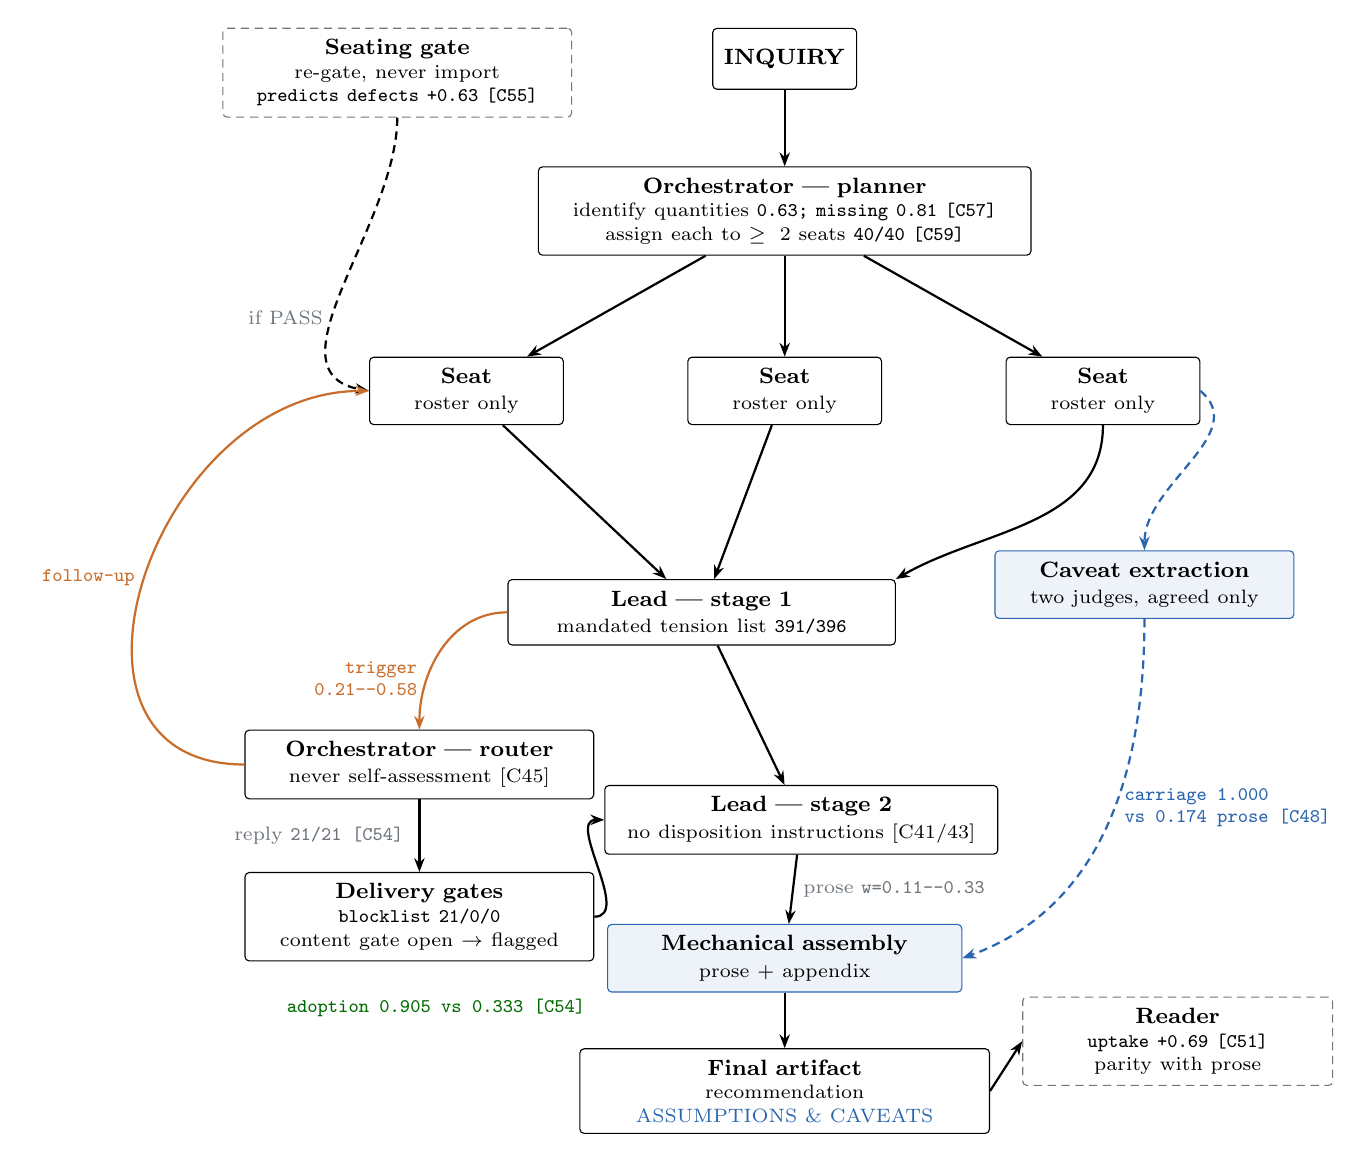
\begin{tikzpicture}[x=1pt,y=1pt,font=\footnotesize,
  box/.style={draw,rounded corners=1.5pt,align=center,inner sep=4pt,minimum height=22pt},
  gate/.style={box,densely dashed,draw=inkmut},
  frt/.style={box,draw=accent,fill=accent!8},
  ed/.style={-{Stealth[length=5pt]},thick},
  edf/.style={-{Stealth[length=5pt]},thick,accent,densely dashed},
  edl/.style={-{Stealth[length=5pt]},thick,corrupt},
  n/.style={font=\scriptsize\ttfamily,text=accent},
  ng/.style={font=\scriptsize\ttfamily,text=black!30!green!60!black},
  nr/.style={font=\scriptsize\ttfamily,text=corrupt},
  s/.style={font=\scriptsize,text=inkmut}]
\node[box] (q) at (170,395) {\textbf{INQUIRY}};
\node[gate,text width=118pt] (sg) at (30,390)
  {\textbf{Seating gate}\\[-1pt]{\scriptsize re-gate, never import}\\[-1pt]
   {\scriptsize\ttfamily predicts defects +0.63 [C55]}};
\node[box,text width=170pt] (pl) at (170,340)
  {\textbf{Orchestrator --- planner}\\[-1pt]
   {\scriptsize identify quantities \ttfamily 0.63; missing 0.81 [C57]}\\[-1pt]
   {\scriptsize assign each to $\ge2$ seats \ttfamily 40/40 [C59]}};
\node[box,text width=62pt] (s1) at (55,275) {\textbf{Seat}\\{\scriptsize roster only}};
\node[box,text width=62pt] (s2) at (170,275) {\textbf{Seat}\\{\scriptsize roster only}};
\node[box,text width=62pt] (s3) at (285,275) {\textbf{Seat}\\{\scriptsize roster only}};
\node[frt,text width=100pt] (cv) at (300,205)
  {\textbf{Caveat extraction}\\{\scriptsize two judges, agreed only}};
\node[box,text width=132pt] (l1) at (140,195)
  {\textbf{Lead --- stage 1}\\{\scriptsize mandated tension list \ttfamily 391/396}};
\node[box,text width=118pt] (rt) at (38,140)
  {\textbf{Orchestrator --- router}\\{\scriptsize never self-assessment [C45]}};
\node[box,text width=118pt] (gt) at (38,85)
  {\textbf{Delivery gates}\\[-1pt]
   {\scriptsize\ttfamily blocklist 21/0/0}\\[-1pt]
   {\scriptsize content gate open $\to$ flagged}};
\node[box,text width=134pt] (l2) at (176,120)
  {\textbf{Lead --- stage 2}\\{\scriptsize no disposition instructions [C41/43]}};
\node[frt,text width=120pt] (asm) at (170,70)
  {\textbf{Mechanical assembly}\\{\scriptsize prose + appendix}};
\node[box,text width=140pt] (fin) at (170,22)
  {\textbf{Final artifact}\\[-1pt]{\scriptsize recommendation}\\[-1pt]
   {\color{accent}\scriptsize ASSUMPTIONS \& CAVEATS}};
\node[gate,text width=104pt] (rd) at (312,40)
  {\textbf{Reader}\\[-1pt]{\scriptsize\ttfamily uptake +0.69 [C51]}\\[-1pt]
   {\scriptsize parity with prose}};
\draw[ed] (q) -- (pl);
\draw[ed,densely dashed] (sg.south) to[out=-90,in=170] node[s,left,pos=.6]{if PASS} (s1.west);
\draw[ed] (pl) -- (s1); \draw[ed] (pl) -- (s2); \draw[ed] (pl) -- (s3);
\draw[ed] (s1) -- (l1); \draw[ed] (s2) -- (l1);
\draw[ed] (s3.south) to[out=-90,in=30] (l1.north east);
\draw[edf] (s3.east) to[out=-40,in=90] (cv.north);
\draw[edf] (cv.south) to[out=-90,in=20]
  node[n,right,pos=.45,align=left]{carriage 1.000\\vs 0.174 prose [C48]} (asm.east);
\draw[edl] (l1.west) to[out=180,in=90]
  node[nr,left,pos=.7,align=right]{trigger\\0.21--0.58} (rt.north);
\draw[edl] (rt.west) to[out=180,in=180,looseness=1.4]
  node[nr,left,pos=.5,align=right]{follow-up} (s1.west);
\draw[ed] (rt) -- node[s,left=2pt]{reply \ttfamily 21/21 [C54]} (gt);
\draw[ed] (gt.east) to[out=0,in=180] (l2.west);
\node[ng] at (44,52) {adoption 0.905 vs 0.333 [C54]};
\draw[ed] (l1) -- (l2);
\draw[ed] (l2) -- node[s,right]{prose \ttfamily w=0.11--0.33} (asm);
\draw[ed] (asm) -- (fin);
\draw[ed] (fin.east) -- (rd.west);
\end{tikzpicture}
\caption{The assembled harness on one inquiry, every edge labeled by its
registered-cell measurement. Dashed blue: the out-of-band freight lane the
writer never sees. Orange: the orchestrator-routed re-consultation loop,
bounded by its measured trigger rate. Seats are interchangeable by
industry --- chairs are earned by the gate, never by category label ---
and engineered overlap between them is where the error immunity lives:
corrupted-value adoption $0.90\to0.45$ [C47], the clean co-source used
end-to-end at $+0.43$ [C59].}
\label{fig:arch}
\end{figure}

\textbf{Seating is empirical, never categorical.} Because signatures
are per-model, no seat is chaired for its category label. A candidate
passes a measured gate: a degeneracy screen ($\ge 800$ visible
characters on screen items --- one archive fine-tune produced $12/12$
degenerate probe runs), a tuned-minus-own-base signature probe, and a
format smoke test at production token budgets. A generalist under a
role prompt is a legitimate seat if it passes; most of our cells ran
on exactly that.

\textbf{Isolation, on cost grounds only.} Seats receive their task and
a one-line roster. Sibling outputs are not forwarded --- but the
original contamination rationale is dead (\S\ref{sec:retests}); the
rule survives because sibling context costs ${\sim}10$k input
characters and $14\%$ longer outputs per seat while buying no measured
change in lane discipline.

\textbf{Redundancy is engineered.} The orchestrator identifies
load-bearing quantities in the decomposition and assigns each to at
least two seats. This is where the council's error immunity lives; it
does not exist by default.

\textbf{Triggers come from mandated artifacts.} The lead runs
two-stage: a mandated tension list first ($391/396$ archived runs
produce one when required), synthesis second. The orchestrator ---
never any model's disposition or self-assessment --- parses the list
and dispatches follow-ups. A reply that adds nothing beyond the seat's
first contribution is dropped, not delivered (a
ritual-effect risk observed at $d\approx0.22$, below our power to
confirm, is treated as live).

\textbf{Epistemic freight travels out-of-band.} Caveats, assumptions,
and confidence never route through the writer: seats emit them as
structured fields and the harness carries them mechanically to an
appendix of the final artifact. The writer receives \emph{no}
disposition instructions at all --- the evidence says they buy nothing
and their surface costs preference.

\textbf{A Goodhart charter.} Trigger rates, hedge counts, compliance
shares, transport slopes, and preference scores on epistemic content
are diagnostics and may never be optimization targets; the optimizable
signal must live outside the pipeline's own text. Each entry on the
forbidden list cites the cell that showed what optimizing it would
manufacture.

\section{The harness attacked: prospective re-tests}
\label{sec:retests}

Design rules distilled from findings can still be wrong --- post-hoc
patterns calcify. So each load-bearing rule got its own registered
cell, with kill conditions stated first. Six verdicts follow.

\textbf{The seating gate predicts (survived).} Ten local candidates
were gated on the frozen degeneracy screen --- two screen items
disjoint from the pipeline case set --- with verdicts committed to the
repository \emph{before} any pipeline run, then every candidate was
seated on the pipeline cases. Strict rank separation held: both
gate-fail candidates defected in the pipeline ($0.333$ and $0.944$ of
contributions) while all eight gate-pass candidates ran at
$0.000$--$0.056$; the pooled contrast is $+0.632$ \ci{+0.549}{+0.722}.
Two refinements rode along: gate verdicts \emph{age} (one model that
passed the archive-era screen failed the fresh re-gate, then defected
in-pipeline at $0.333$ --- seating must re-gate, never import a stored
verdict), and format compliance is a separate axis that does not
predict seat defects (the legal fine-tune failed the format smoke $0/4$
yet seated defect-free; that component's proper target is
verdict-emitting roles).

\textbf{Redundancy is causal (survived).} One factor --- assign the
contested quantity to a second seat --- halved corrupted-value
adoption, $0.900\to0.450$ (\ci{+0.200}{+0.725}), with the clean value
actually adopted ($0.000\to0.500$): selection, not dilution. The bare
arm's $0.900$ doubles as the sharpest no-verification number on
record. Protection is bimodal across items; two candidate boundary
mechanisms were then registered and killed (prior-plausibility at
$0.544$; the elicited ownership map at exactly $0.500$ prospective
against $0.895$ descriptive, with an MDD of $0.68$ --- the
confirmation cell doing its anti-calcification job). The boundary is
OPEN and stated as such.

\begin{figure}[t]
\centering
\begin{minipage}{0.44\textwidth}
\centering
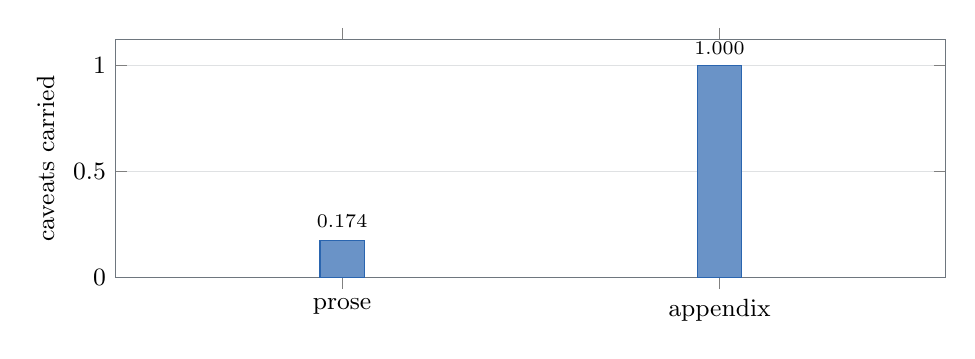
\begin{tikzpicture}
\begin{axis}[width=\textwidth,height=4.6cm,ybar,bar width=16pt,
  ymin=0,ymax=1.12,xtick={1,2},xticklabels={prose,appendix},
  ylabel={caveats carried},xmin=0.4,xmax=2.6,
  tick label style={font=\small},ylabel style={font=\small},
  axis line style={inkmut},ymajorgrids,grid style={inkmut!22}]
\addplot+[fill=accent!70,draw=accent] coordinates {(1,0.174) (2,1.000)};
\node[font=\scriptsize,anchor=south] at (axis cs:1,0.19) {0.174};
\node[font=\scriptsize,anchor=south] at (axis cs:2,1.005) {1.000};
\end{axis}
\end{tikzpicture}
\end{minipage}\hfill
\begin{minipage}{0.53\textwidth}
\centering
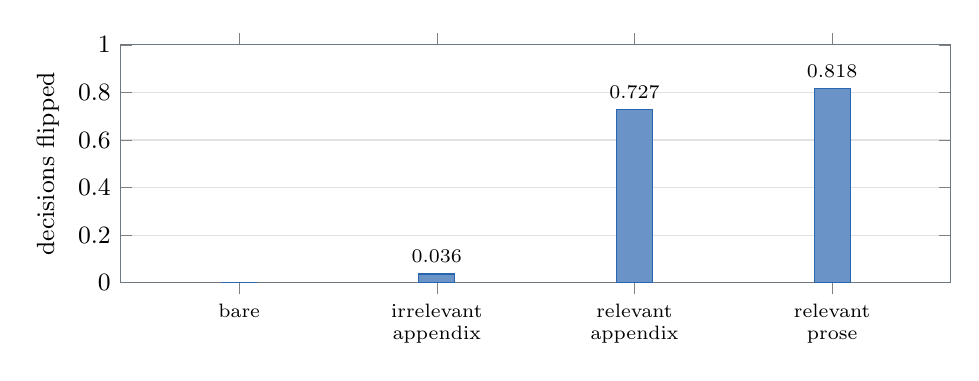
\begin{tikzpicture}
\begin{axis}[width=\textwidth,height=4.6cm,ybar,bar width=13pt,
  ymin=0,ymax=1.0,xtick={1,2,3,4},
  xticklabels={bare,{irrelevant\\appendix},{relevant\\appendix},
  {relevant\\prose}},xticklabel style={font=\scriptsize,align=center},
  ylabel={decisions flipped},xmin=0.4,xmax=4.6,
  tick label style={font=\small},ylabel style={font=\small},
  axis line style={inkmut},ymajorgrids,grid style={inkmut!22}]
\addplot+[fill=accent!70,draw=accent] coordinates
  {(1,0.000) (2,0.036) (3,0.727) (4,0.818)};
\node[font=\scriptsize,anchor=south] at (axis cs:2,0.045) {0.036};
\node[font=\scriptsize,anchor=south] at (axis cs:3,0.732) {0.727};
\node[font=\scriptsize,anchor=south] at (axis cs:4,0.823) {0.818};
\end{axis}
\end{tikzpicture}
\end{minipage}
\caption{The out-of-band channel, attacked on both halves and
surviving. \emph{Left}: caveat carriage through writer prose vs.\ the
mechanically assembled appendix (zero-generation design). \emph{Right}:
registered two-token reader decisions flipped by a planted
decision-relevant caveat, by delivery arm; the irrelevant-appendix
control shows the effect is content, not appendix-presence. Uptake
$+0.691$ \ci{+0.455}{+0.891}; parity with prose $+0.091$
\ci{-0.036}{+0.218}.}
\label{fig:freight}
\end{figure}

\textbf{Out-of-band freight carries and is used (survived).} Carriage:
the appendix delivers $1.000$ of both-judge caveat sentences against
$0.174$ surviving prose, with no detected preference penalty ($0.510$
\ci{0.267}{0.754}; not evaluable at power, reported as bounded).
Uptake: appendix-delivered caveats flip a reader's registered decision
at $0.727$ against $0.036$ for the identical block carrying an
irrelevant caveat, with direction-balanced items so caution cannot
masquerade as uptake, at parity with in-prose placement
(Figure~\ref{fig:freight}). The channel preference cannot see is not
an exhibit; it changes decisions.

\textbf{The live loop closes (survived, with one halt en route).} A
first live-specialist cell buried the deciding fact in the
specialist's own round-one text and \emph{halted at its registered
pilot gate}: the trigger named the tension at only $0.208$ with the
fact visible in the pile. The redesign supplied the fact as the
specialist's private working notes --- knowledge held but never
written --- and restored the original round-one bytes. The live
specialist conveyed the fact $21/21$ when dispatched; the lead adopted
at $0.905$ vs.\ $0.333$ archived control ($+0.571$
\ci{+0.139}{+0.912}), within $-0.095$ \ci{-0.227}{0.000} of the
scripted ceiling. One new risk is on record: $4/21$ live replies
embellished the correctly conveyed fact with \emph{fabricated}
authority --- invented case law, invented regulatory rulings --- and
were adopted anyway. Content gates screen absence, not invention; the
fabrication rate is observed, not bounded.

\textbf{Isolation lost its warrant (demoted).} The registered
one-factor test made byte-fixed sibling contributions visible under
production prompts: off-domain framework density moved $-0.009$
\ci{-0.048}{+0.028} against a pre-registered MDD of $+0.05$--$0.08$
computed from the archive --- an informative null, with in-domain
density unchanged. The contamination rationale is withdrawn; the rule
stands on cost. (A registered secondary even pointed the other way:
seats shown their siblings' coverage used slightly \emph{fewer}
off-domain terms of their own, $-0.033$ \ci{-0.053}{-0.013} ---
recorded as a candidate mechanism, not claimed.)

\textbf{The ownership law died in confirmation (killed).} A stable,
near-unanimous elicited map of which seat ``owns'' each quantity ---
exactly the kind of pattern a framework would ship as a routing table
--- predicted arbitration at chance on fresh items. We report this
kill with the survivals because it is the argument: the difference
between an evidence-bound harness and a prompt stack is that the
harness can lose these arguments in public, on the record, component
by component.

\section{Operating economics and open risks}
\label{sec:economics}

\textbf{The trigger bounds coverage.} Everything downstream of the
trigger is now measured and works; the trigger itself fires at
$0.208$--$0.583$ by batch and is deliberately not an optimization
target (raising it blind manufactures the ritual condition the loop's
own control arm exposed). Deployments should budget coverage
accordingly: the loop resolves the contested quantities it notices,
and it does not notice most of them.

\textbf{Open risks, stated.} Per-item protection is bimodal with the
boundary mechanism unknown (two candidates killed). Live-reply
fabrication is now \emph{bounded} by a registered follow-up cell:
reply-level $0.100$ \ci{0.047}{0.201} with the deciding fact in hand,
$0.150$ \ci{0.081}{0.261} without it --- concentrated entirely on one
trigger topic ($15/20$ there, $0/100$ elsewhere) and name-stable, the
same two invented decisions recurring across independent samples,
which licenses a blocklist delivery filter; the seat never admits the
gap ($0/20$ sampled), the backfill mechanism is directionally positive
but not evaluable at six clusters, and the bound covers adversarial
case citations only --- a floor, not a ceiling, on confabulation. The
preference cost of the appendix is bounded-not-evaluable at current
power; and the council's accuracy question remains absence-of-evidence
on the program's weakest surviving row. None of these is hidden in the
architecture document; each is attached to the component it concerns.

\textbf{Running the harness replicates the science.} The harness's
telemetry doubles as a replication battery: every deployment yields
transport estimates, trigger telemetry, phrase-swap slots for proposed
instructions, and preference-vs-verified divergence wherever ground
truth exists --- each with its attainability gate. An honest
deployment is also, at near-zero marginal cost, the external
validation the program's scope caveats call for.

\section{Related work}
\label{sec:related}

MoA \cite{wang2024moa} and successors report preference gains from
aggregation; Self-MoA \cite{li2025selfmoa} shows mixing weaker models
often hurts, consistent with our per-model signature result. Debate
and multi-agent-discussion results \cite{wang2024rebuttal} find gains
concentrated where prompts were weak, consistent with our finding that
the one working intervention routes \emph{information}, not
deliberation. LLM-judge critiques \cite{zheng2023judging} motivate our
order-debiased two-family protocol; length and sycophancy pressure
\cite{singhal2023length,sharma2023sycophancy} sharpen to our measured
phrase penalty. We are not aware of prior work that pre-registers each
component of a multi-agent architecture and reports the failures with
the survivals; that practice, more than any single component, is what
we propose for adoption.

\section{Limitations}
\label{sec:limits}

Scale and scope: 7--20B local models, advisory-domain English, one
primary writer family (cross-family replications where stated).
Cluster ceilings of 6--18 items bind every harness cell; the live-loop
comparison uses archived arms under a registered fresh-batch check;
the uptake verdict covers 11 of 18 authored items after a registered
floor gate; trigger rates are batch-variable and quoted only as a
range. The harness's gains are preference, immunity, and resolution
--- \emph{not} accuracy, which remains untested at the standard the
program set for itself. Verdicts inherit their cells' scope and should
not be generalized past it; the architecture document states, for
every component, exactly which cell licenses it.

\section{Reproducibility}

The complete pre-registration ledger (52 registration blocks at this
writing), every deviation and verdict including the two halts, the
architecture document, the measurement kit (\texttt{gst}), the frozen
dictation registry, and all item files are in the project repository;
registrations are committed before first runs, so temporal ordering is
verifiable from history.

\begin{thebibliography}{9}
\bibitem{wang2024moa} J.~Wang, J.~Wang, B.~Athiwaratkun, C.~Zhang,
J.~Zou. Mixture-of-Agents enhances large language model capabilities.
\emph{arXiv:2406.04692}, 2024.
\bibitem{bobo2026audit} S.~Bobo. Instructions buy the phrase; the
phrase costs preference: an epistemic audit of LLM aggregation
pipelines at auditable scale. Companion draft, 2026.
\bibitem{li2025selfmoa} W.~Li et al. Rethinking Mixture-of-Agents: is
mixing different large language models beneficial?
\emph{arXiv:2502.00674}, 2025.
\bibitem{zheng2023judging} L.~Zheng et al. Judging LLM-as-a-judge with
MT-Bench and Chatbot Arena. \emph{NeurIPS Datasets and Benchmarks},
2023.
\bibitem{singhal2023length} P.~Singhal et al. A long way to go:
investigating length correlations in RLHF. \emph{arXiv:2310.03716},
2023.
\bibitem{sharma2023sycophancy} M.~Sharma et al. Towards understanding
sycophancy in language models. \emph{arXiv:2310.13548}, 2023.
\bibitem{wang2024rebuttal} Q.~Wang et al. Rethinking the bounds of LLM
reasoning: are multi-agent discussions the key?
\emph{arXiv:2402.18272}, 2024.
\end{thebibliography}

\end{document}
